\documentclass[32pt, aspectratio = 169]{beamer}

\usepackage[utf8]{inputenc} % Character encoding.

\pdfinfo{
   /Author (Bashar Dudin)
   /Title  (The Simplex Algorithm I)
   /Subject (Linear Programs)
}


\usepackage{./Style/linearProgramsBeamer} % This is extra styling for Beamer environments.
\usepackage{./Style/linearProgramsStyle} % This is a set of commands for maths content.

%-------------------------------------------------------------------------------
%   TITLE PAGE
%-------------------------------------------------------------------------------

\author[BD]{Bashar Dudin}

\institute[]{EPITA}

\title{Linear Programs} %
\subtitle{The Simplex Algorithm I}

%-------------------------------------------------------------------------------
%   DOCUMENT BODY
%-------------------------------------------------------------------------------

\begin{document}

\begin{frame}[plain]
\titlepage % Print the title page as the first slide
\end{frame}

\section{Linear Optimization over Polyhedra}

\begin{frame}{Geometry of the Set of Feasible Solutions}
    Let $L$ be the following linear program, in standard form :
    \begin{figure}
        \begin{linearProg}{
            maximize
            }{
            $x_1 + 2x_2$
            }{
            \systeme{x_1 + x_2 \leq 5, -2x_1 + x_2 \leq 3}
            }{
            $x_1, x_2 \geq 0$
            }
        \end{linearProg}
    \end{figure}

    The set of feasible solutions of $L$ is the region of the plane in
    between the positive parts of both axes and the lines having
    equations $x_2 = 5 - x_1$ and $x_2 = 3 + 2x_1$.
\end{frame}

\begin{frame}{Geometry of the Set of Feasible Solutions}
  \begin{columns}
    \begin{column}{.4\textwidth}
      This set of feasible solutions of $L$ has a remarkable geometric
      property called \textit{convexity}.
      \begin{defn}
        A subset $A$ of $\R^n$ is said to be \emph{convex} if the
        line segment linking any two points of $A$ is contained in
        $A$.
      \end{defn}
      In our case, we have a specific type of convex set called a
      \emph{polyhedron}. It is the intersection of a finite set of
      half-spaces.
    \end{column}
    \begin{column}{.6\textwidth}
      \begin{figure}
        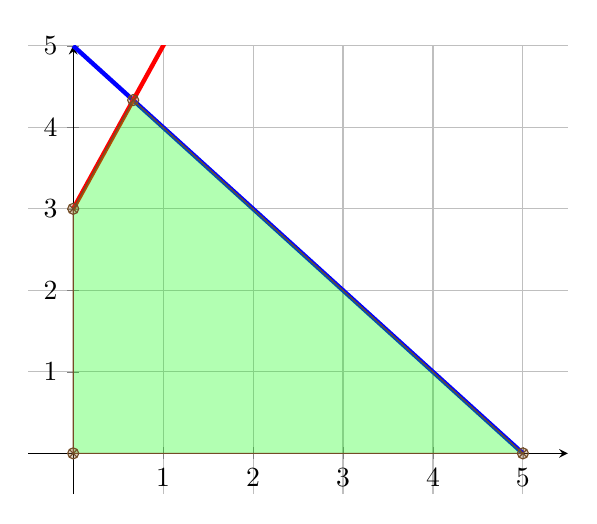
\begin{tikzpicture}
          \begin{axis}[
            domain=0:5, xmin=-0.5, xmax=5.5, ymin=-0.5, ymax=5,
            grid=major, axis x line=center, axis y line=center,
            legend pos=north east,
            ]
            \addplot+[ultra thick, mark = none] {5 - x};
            \addplot+[ultra thick, mark = none] {3 + 2*x};
            \addplot+[fill = green, fill opacity = 0.3] coordinates
            {(0,0) (0,3) (.667,4.334) (5,0)} \closedcycle ;
          \end{axis}
        \end{tikzpicture}
      \end{figure}
    \end{column}
  \end{columns}
\end{frame}

\begin{frame}{Geometry of the Set of Feasible Solutions}
  \begin{prop}
    Any linear program has an underlying set of feasible solutions
    which is convex.
  \end{prop}
  \begin{defn}
    We call \emph{interior} of a convex set $A$ the set of points
    $x \in A$ for which there is a disk having a positive radius and
    centered at $x$ contained in $A$. Any point of $A$ not satisfying
    this condition is called a \emph{boundary point}. The
    \emph{boundary} of $A$ is the set of boundary points.
  \end{defn}
  When dealing with convex sets defined by linear constraints,
  boundary points are points of the hyperplanes defined by replacing
  inequalities by equalities. This is clearly the case in our
  $2$-dimensional case.
\end{frame}

\begin{frame}{Boundary Optimizes Linear Function}
  Recall that a function $f : A \to \R$ for a region $A$ in $\R^n$ is
  said to be \emph{bounded} if there is a positive real number $M$
  such that : for all $x \in A$, $\Big|f(x)\Big| \leq M$.
  \begin{prop}
    Let $A$ be the region defined by the set of feasible solutions of
    a linear program $L$. If the objective functional is
    \textit{bounded} on $A$ then $L$ has an optimal objective value,
    it is attained on the boundary of $A$.
    \end{prop}
\end{frame}

\begin{frame}
  \frametitle{Boundary Optimizes Linear Function | Naive Search}
  %% TODO: Write down the intersection case, make a quick computation
  %% of generic number of intersection points.
\end{frame}

\begin{frame}{Boundary Optimizes Linear Function | A Better Search}
  Rather than listing all potential optimal points, the \emph{simplex
    algorithm} is a walk along boundary points of the feasible region
  satisfying the fact :
  \begin{quotation}
    A given step has higher or equal objective value than previous
    step.
  \end{quotation}
  It has an initialization step, that we're going to keep on the side
  for now. \pause We shall be working under the following assumption.
  \begin{alertblock}{Assumption}
    Given a linear program $L$ in \textit{standard} form, we assume
    the vector having only zero entries is a feasible solution of $L$.
  \end{alertblock}
  In the following example, starting from the zero feasible solution
  we're going to walk around the boundary of the feasible region to
  look for an optimal value.
\end{frame}

\section{Simplex Algorithm : First Try}


\begin{frame}{Simplex Algorithm : First Practical Examples}
    This is the slack form of the linear program $L$ we started with:
    \begin{figure}
      \begin{linearProg}{
          maximize
        }{
          $x_1 + 2x_2$
        }{
          \systeme{x_3 = 5 - x_1 - x_2, x_4 = 3 + 2x_1 - x_2 }
        }{
          $x_1, x_2, x_3, x_4 \geq 0$
        }
      \end{linearProg}
    \end{figure}
    The zero feasible solution of the standard form of $L$ corresponds
    to the solution $(0, 0, 5, 3)$ of its slack form; it has objective
    value $0$. The slack variables $x_3$ and $x_4$ tell us how far
    solution $(x_1, x_2)$ is from making the constraints
    \[
    \sysdelim..{\systeme{x_1 + x_2 \leq 5, -2x_1 + x_2 \leq 3}}
    \]
    tight, i.e. equalities.
\end{frame}

\begin{frame}{Simplex Algorithm : First Practical Examples}
    \begin{columns}
        \begin{column}{.5\textwidth}
            \begin{onlyenv}<1
              >The feasible slack solution of $(0, 0, 5, 3)$ has
              corresponding feasible standard solution the origin of
              the plane. To wander around the boundary of the feasible
              region we have to choose which way to go; we either go
              vertically keeping $x_1$ to $0$ or horizontally keeping
              $x_2$ to $0$. Any choice is fine as long as we are
              increasing the objective value. We shall give a
              \textit{rule of thumb} as to what choice one can make at
              each step later. For now, let us increase $x_1$ while
              keeping $x_2$ at $0$.
            \end{onlyenv}
            \begin{onlyenv}<2
              >
              \begin{figure}
                \begin{linearProg}{
                    maximize
                  }{
                    $x_1 + 2x_2$
                  }{
                    \systeme{x_3 = 5 - x_1 - x_2, x_4 = 3 + 2x_1 - x_2 }
                  }{
                    $x_1, x_2, x_3, x_4 \geq 0$  %% TODO: maths spacing
                  }
                \end{linearProg}
              \end{figure}
              $x_1$ is constrained by the first equation: increasing
              $x_1$ indefinitely would violate non-negativity
              constraints while no such constraints come from the
              second equation. The highest possible value for $x_1$ is
              thus obtained when $x_3$ is zero. The resulting feasible
              solution is $(5, 0, 0, 13)$, of objective value
              $5$. Corresponding solution of standard form is tight
              for first constraint.
            \end{onlyenv}
            \begin{onlyenv}<3
              >To get the feasible solution $(5, 0, 0, 13)$ one can
              express $x_1$ in the first equation in terms of the two
              other variables. One then replaces $x_1$ elsewhere with
              this expression. We get the equivalent program
                \begin{figure}
                \begin{linearProg}{
                        maximize
                        }{
                        $5 - x_3 + x_2$
                        }{
                        \systeme{x_1 = 5 - x_3 - x_2, x_4 = 13 - 2x_3 - 3x_2 }
                        }{
                        $x_1, x_2, x_3, x_4 \geq 0$
                        }
                \end{linearProg}
                \end{figure}
                Putting $x_3$ and $x_2$ to zero in both equation gives
                back the expected feasible solution.
            \end{onlyenv}
            \begin{onlyenv}<4-5
                >\alt<5>{
                \textcolor{orange}{
                \begin{figure}
                \begin{linearProg}{
                        maximize
                        }{
                        $\dfrac{28}{3} - \dfrac{5}{3}x_3 - \dfrac{1}{3}x_4$
                        }{
                        \systeme{x_1 = 2/3 - (1/3)x_3 + (1/3) x_4, x_2 = 13/3 - (2/3)x_3 - (1/3)x_4 }
                        }{
                        $x_1, x_2, x_3, x_4 \geq 0$
                        }
                \end{linearProg}
                \end{figure}
                }
                \vspace{-1em}
                Playing the same previous trick using $x_2$ and the second equation we get the above equivalent linear program. Putting both $x_3$ and $x_4$ to zero, we get the feasible solution $(2/3, 13/3, 0, 0)$ which has objective value $28/3$.
                }{
                \begin{figure}
                \begin{linearProg}{
                        maximize
                        }{
                        $5 - x_3 + x_2$
                        }{
                        \systeme{x_1 = 5 - x_3 - x_2, x_4 = 13 - 2x_3 - 3x_2 }
                        }{
                        $x_1, x_2, x_3, x_4 \geq 0$
                        }
                \end{linearProg}
                \end{figure}
                One can hope to maximize this linear program by increasing $x_2$. Any increase in $x_3$ would decrease the objective value. The most restrictive equation for $x_2$ is the second, indeed one can only increase $x_2$ up to $13/3$ while in the second up to $5$.
                }
            \end{onlyenv}
            \begin{onlyenv}<6->
                \begin{figure}
                \begin{linearProg}{
                        maximize
                        }{
                        $\dfrac{28}{3} - \dfrac{5}{3}x_3 - \dfrac{1}{3}x_4$
                        }{
                        \systeme{x_1 = 2/3 - (1/3)x_3 + (1/3) x_4, x_2 = 13/3 - (2/3)x_3 - (1/3)x_4 }
                        }{
                        $x_1, x_2, x_3, x_4 \geq 0$
                        }
                \end{linearProg}
                \end{figure}
                \vspace{-1em}
                We can't hope to increase the objective value. Any increase in the values of $x_3$ or $x_4$ would decrease the object value. The objectve function is maximal when both are zero. The corresponding maximal solution is $(2/3, 13/3, 0, 0)$ of objective value $28/3$.
            \end{onlyenv}
        \end{column}
        \begin{column}{.5\textwidth}
            \begin{overlayarea}{\textwidth}{.8\textheight}
                \begin{onlyenv}<1>
                \begin{figure}
                    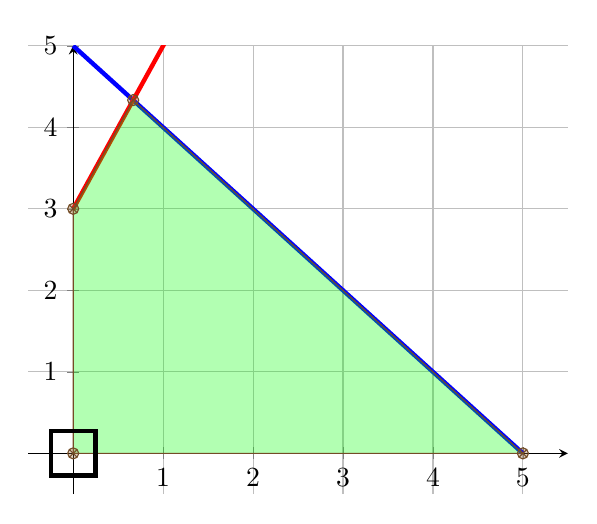
\begin{tikzpicture}
                        \begin{axis}[
                            domain=0:5, xmin=-0.5, xmax=5.5, ymin=-0.5, ymax=5,
                            grid=major, axis x line=center, axis y line=center,
                            legend pos=north east,
                            ]
                            \addplot+[ultra thick, mark = none] {5-x};
                            \addplot+[ultra thick, mark = none] {3 + 2*x};
                            \addplot+[fill = green, fill opacity = 0.3] coordinates
                            {(0,0) (0,3) (.667,4.334) (5,0)} \closedcycle ;
                            \addplot[ultra thick, black, mark size = 8pt, mark = square] coordinates {(0,0)};
                        \end{axis}
                    \end{tikzpicture}
                \end{figure}
                \end{onlyenv}
                \begin{onlyenv}<2-4>
                    \begin{figure}
                    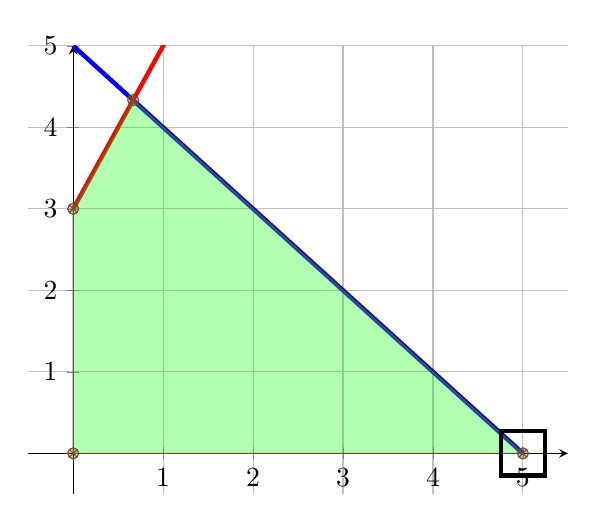
\begin{tikzpicture}
                        \begin{axis}[
                            domain=0:5, xmin=-0.5, xmax=5.5, ymin=-0.5, ymax=5,
                            grid=major, axis x line=center, axis y line=center,
                            legend pos=north east,
                            ]
                            \addplot+[ultra thick, mark = none] {5-x};
                            \addplot+[ultra thick, mark = none] {3 + 2*x};
                            \addplot+[fill = green, fill opacity = 0.3] coordinates
                            {(0,0) (0,3) (.667,4.334) (5,0)} \closedcycle ;
                            \addplot[ultra thick, black, mark size = 8pt, mark = square] coordinates {(5,0)};
                        \end{axis}
                    \end{tikzpicture}
                \end{figure}
                \end{onlyenv}
                \begin{onlyenv}<5->
                    \begin{figure}
                    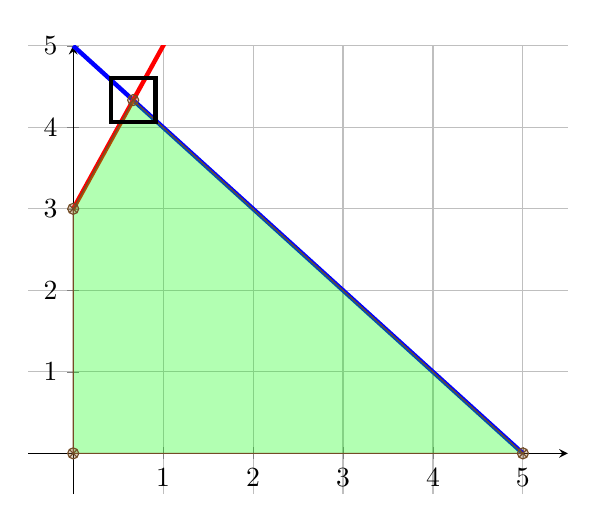
\begin{tikzpicture}
                        \begin{axis}[
                            domain=0:5, xmin=-0.5, xmax=5.5, ymin=-0.5, ymax=5,
                            grid=major, axis x line=center, axis y line=center,
                            legend pos=north east,
                            ]
                            \addplot+[ultra thick, mark = none] {5-x};
                            \addplot+[ultra thick, mark = none] {3 + 2*x};
                            \addplot+[fill = green, fill opacity = 0.3] coordinates
                            {(0,0) (0,3) (.667,4.334) (5,0)} \closedcycle ;
                            \addplot[ultra thick, black, mark size = 8pt, mark = square] coordinates {(.667, 4.334)};
                        \end{axis}
                    \end{tikzpicture}
                    \end{figure}
                \end{onlyenv}
            \end{overlayarea}
        \end{column}
    \end{columns}
\end{frame}

\section{Simplex Algorithm : A Step Towards Rigorousness}

\begin{frame}{Notation and Terminology}
    Consider a linear program given in standard form as
    \begin{figure}
        \begin{linearProgG}{
            ${\displaystyle z = \nu + \sum_{j=1}^n c_jx_j}$
            }{
            ${\displaystyle \forall i \in B, \quad \sum_{j=1}^n a_{ij}x_j \leq b_i}$
            }{
            $\forall j \in N, \quad x_j \geq 0$
            }
        \end{linearProgG}
    \end{figure}
    where $(a_{ij})_{i, j}$ is an $(m, n)$ matrix. The set $N$ is the set $\{ 1, \ldots, n \}$ of indexes of variables, the one of $B$ is the set $\{ n+1, \ldots, n+m \}$ indexing linear constraints. The need for these two sets will be clear later on. Lastly, $(c_1, \ldots, c_n)$ is a vector of size $n$ while $(b_{n+1}, \ldots, b_{n+m})$ is one of size $m$.
\end{frame}

\begin{frame}{Notation and Terminology}
    The slack form of the previous linear program is written
    \begin{figure}
        \begin{linearProgG}{
            ${\displaystyle z = \nu + \sum_{j=1}^n c_jx_j}$
            }{
            ${\displaystyle \forall i \in B, \quad x_i = b_i - \sum_{j=1}^n a_{ij}x_j}$
            }{
            $\forall j \in N\cup B, \quad x_j \geq 0$
            }
        \end{linearProgG}
    \end{figure}
    The set of variables on the left (and indexed by $B$) are called \emph{basic} variables. Variables on the left and indexed by $N$ are called \emph{non-basic} ones. The \emph{basic solution} of a linear program in slack form is the one obtained by putting all non-basic variables to zero. This is not, in general, a feasible solution of the linear program (but we'll learn to deal with it).
\end{frame}

\begin{frame}{Practical Steps of the Simplex Algorithm}
    The simplex algorithm is a procedure exchanging a basic variable with a non-basic one at each step. Recall that up so far we have been working under the following assumption:
    \begin{alertblock}{Assumption}
        The zero tuple is a feasible solution of the linear program in standard form. Equivalently, the \textit{basic solution} of the slack form of our linear program is a feasible solution.
    \end{alertblock}
    We shall take care of the general case later. It does build up on this case.
\end{frame}

\begin{frame}{Practical Steps of the Simplex Algorithm}
    Here is the main steps of the simplex algorithm
    \begin{itemize}
        \item[\textbullet] Choose a non-basic variable $x_e$ increasing the objective value.
        \item[\textbullet] Use the most restrictive constraint $\ell$ on $x_e$ to express $x_e$ in terms of the remaining variables.
        \item[\textbullet] Replace $x_e$ in remaining linear equalities and linear functional by the expression previously obtained. The variable $x_e$ becomes a basic variable while $x_\ell$ becomes non-basic.
        \item[\textbullet] Putting all non-basic variables to zero we get a tuple whose first $n$ entries are a feasible solution of the linear program we started with.
        \item[\textbullet] Repeat previous steps until there is no room for increasing the objective value.
    \end{itemize}
\end{frame}

\begin{frame}{Practical Steps of the Simplex Algorithm}
    The previous steps are precisely what we've been doing while wandering around the boundary of our case. This approach does however exceed the $2$-dimensional case.
    \begin{halfshyblock}{A $3$-dimensional case}
        Following previous steps try solving the linear program
         \begin{figure}
        \begin{linearProg}{
            maximize
            }{
            $3x_1 + x_2 + 2x_3 $
            }{
            \systeme{x_1 + x_2 + 3x_3 \leq 30, 2x_1 + x_2 + 5x_3 \leq 24, 4x_1 + x_2 + x_3 \leq 36}
            }{
            $x_1, x_2, x_3 \geq 0 $
            }
        \end{linearProg}
    \end{figure}
    \end{halfshyblock}
\end{frame}
\begin{frame}{A Finishing Blow about Boundedness}
    Notice that there is no garantee that the previous algorithm would get you a maximal solution in general. We do know that, if the linear functional is bounded on the feasible region, then there is a maximum attained at the boundary of this region. But there are cases when the linear functional is not bounded on the feasible region.
    \begin{halfshyblock}{Unboundedness}
        Can you find a linear program which is not bounded?
    \end{halfshyblock}
\end{frame}

\begin{frame}
  \begin{center}
    {\huge \textbf{That's it for today}}
   \end{center}
 \end{frame}

%%%%%%%%%%%%%%%%%%%%%%%%%%%%%%%%%%%%%%%%%%%%%%%%%%%%%%%%%%%%%%%

\end{document}


%%% Local Variables:
%%% mode: latex
%%% TeX-master: t
%%% End:
